\section{Proposed Solution}

The events of a trace will be transformed into a node-link graph. One possible idiom for trace comparison, is to compare the graphs formed by the events of different traces
by partitioning them into side-by-side views. Another possible idiom is showing the diff of the 2 graphs whilst still preserving
the original graphs to provide some sort of context.
Because of the limited screen space of a computer monitor, we will allow at most two
graphs to be compared at one time. Even though our tool will only allow two graphs to be compared at once, users will still be able
to compare multiple traces by aggregating traces that go through the exact same nodes into one graph. In other words, traces that have
the same structure can be aggregated into one graph. This aggregation procedure will allow us to make comparisons that involve many
traces while only using two DAGs. The links of the graph will be saturated according to the average time it takes for the event in
the end of the link to complete. We will also use colour hue to identify the \textit{process\_name} of each event. A preliminary sketch of
this visualization can be seen in Figure \ref{fig:comparison}.

We will use a similar approach to create the service dependency graph. To create the dependency graph for one trace, we will transform the list
of events into a DAG represented by a node-link graph. All the events with the same \textit{process\_name} will be aggregated into the same
node. In this representation, the aggreated node will represent a service in a microservice. The links to the node will be saturated according
to the amount of time it takes for all the events in a service to complete. A preliminary sketch of this visualization can be seen in Figure \ref{fig:aggregation}.

At the moment, our proposed solution for source code integration does not have a specific visualization in mind. We are thinking about
providing a link to the file and line in the github repo corresponding to the selected event in a trace. At least initially, we are not
going to do any complicated visualization to accomplish the source code integration task.

\begin{figure}
    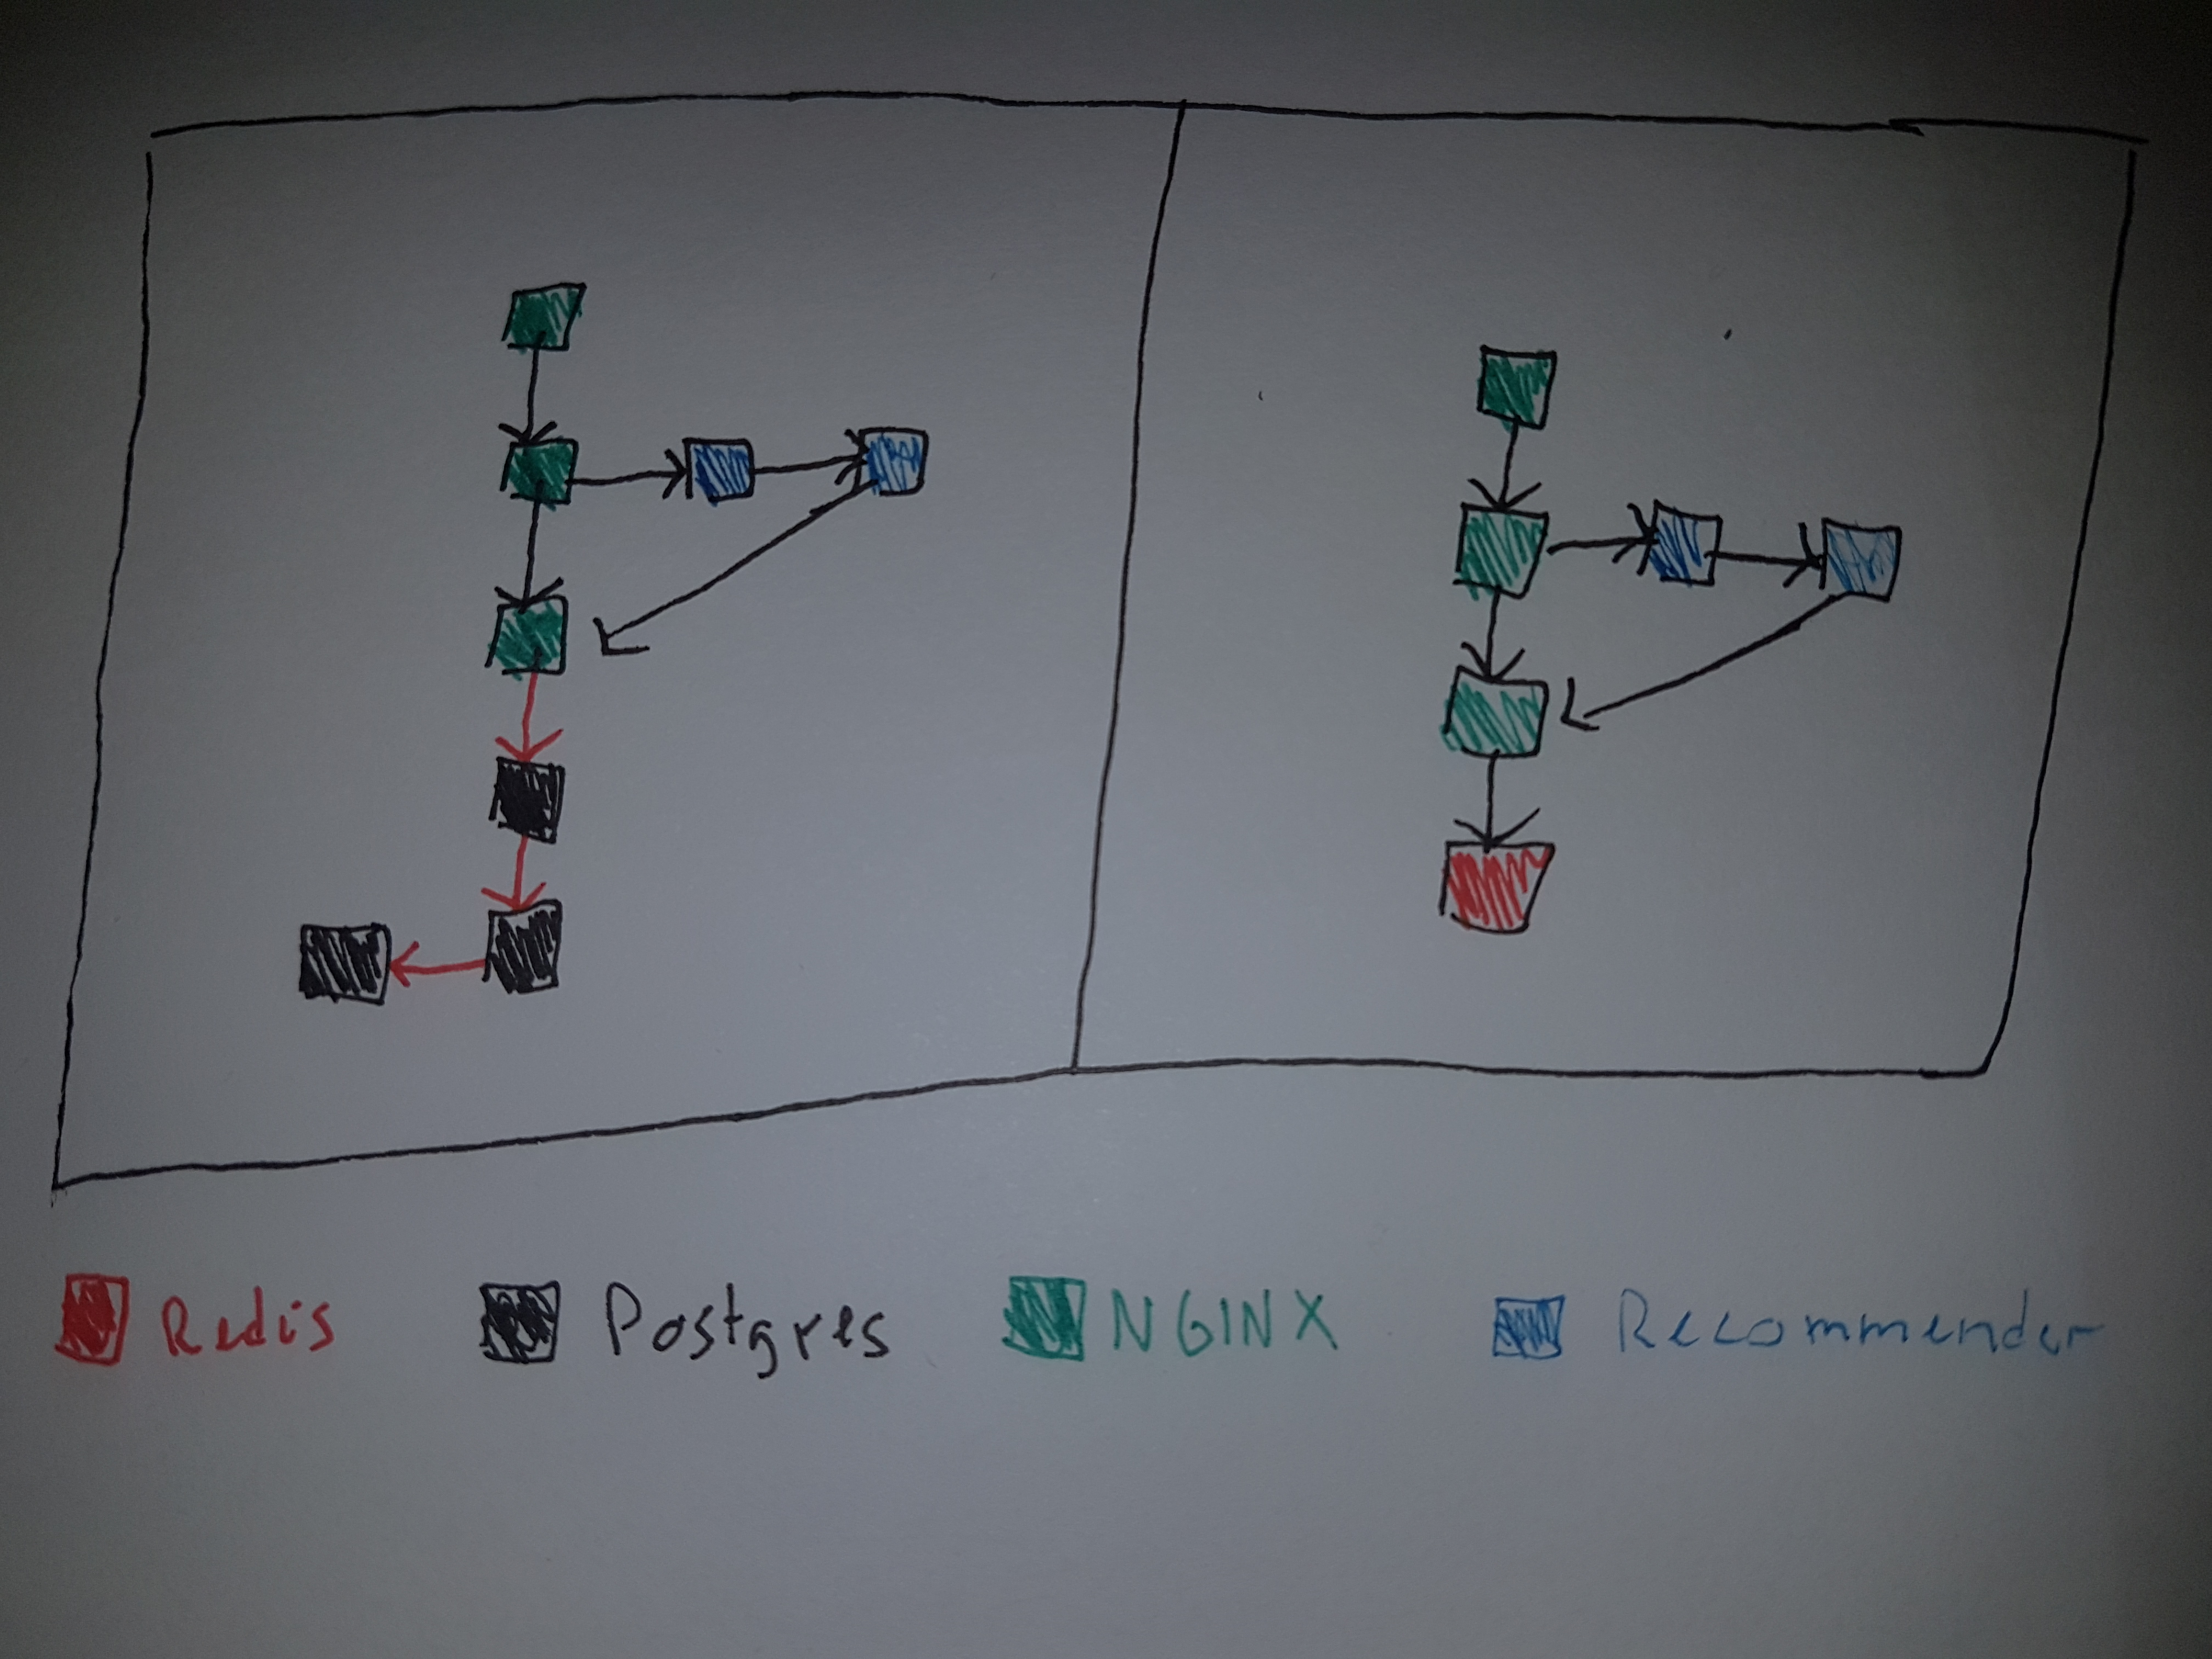
\includegraphics[width=\linewidth]{comparison.jpg}
    \caption{Example of a comparison task where we compare one task that calls Postgres and another that calls Redis. The trace that
    called Postgres triggers slow events (represented by the red links) and triggers more events in general.}
    \label{fig:comparison}
\end{figure}

\begin{figure}
    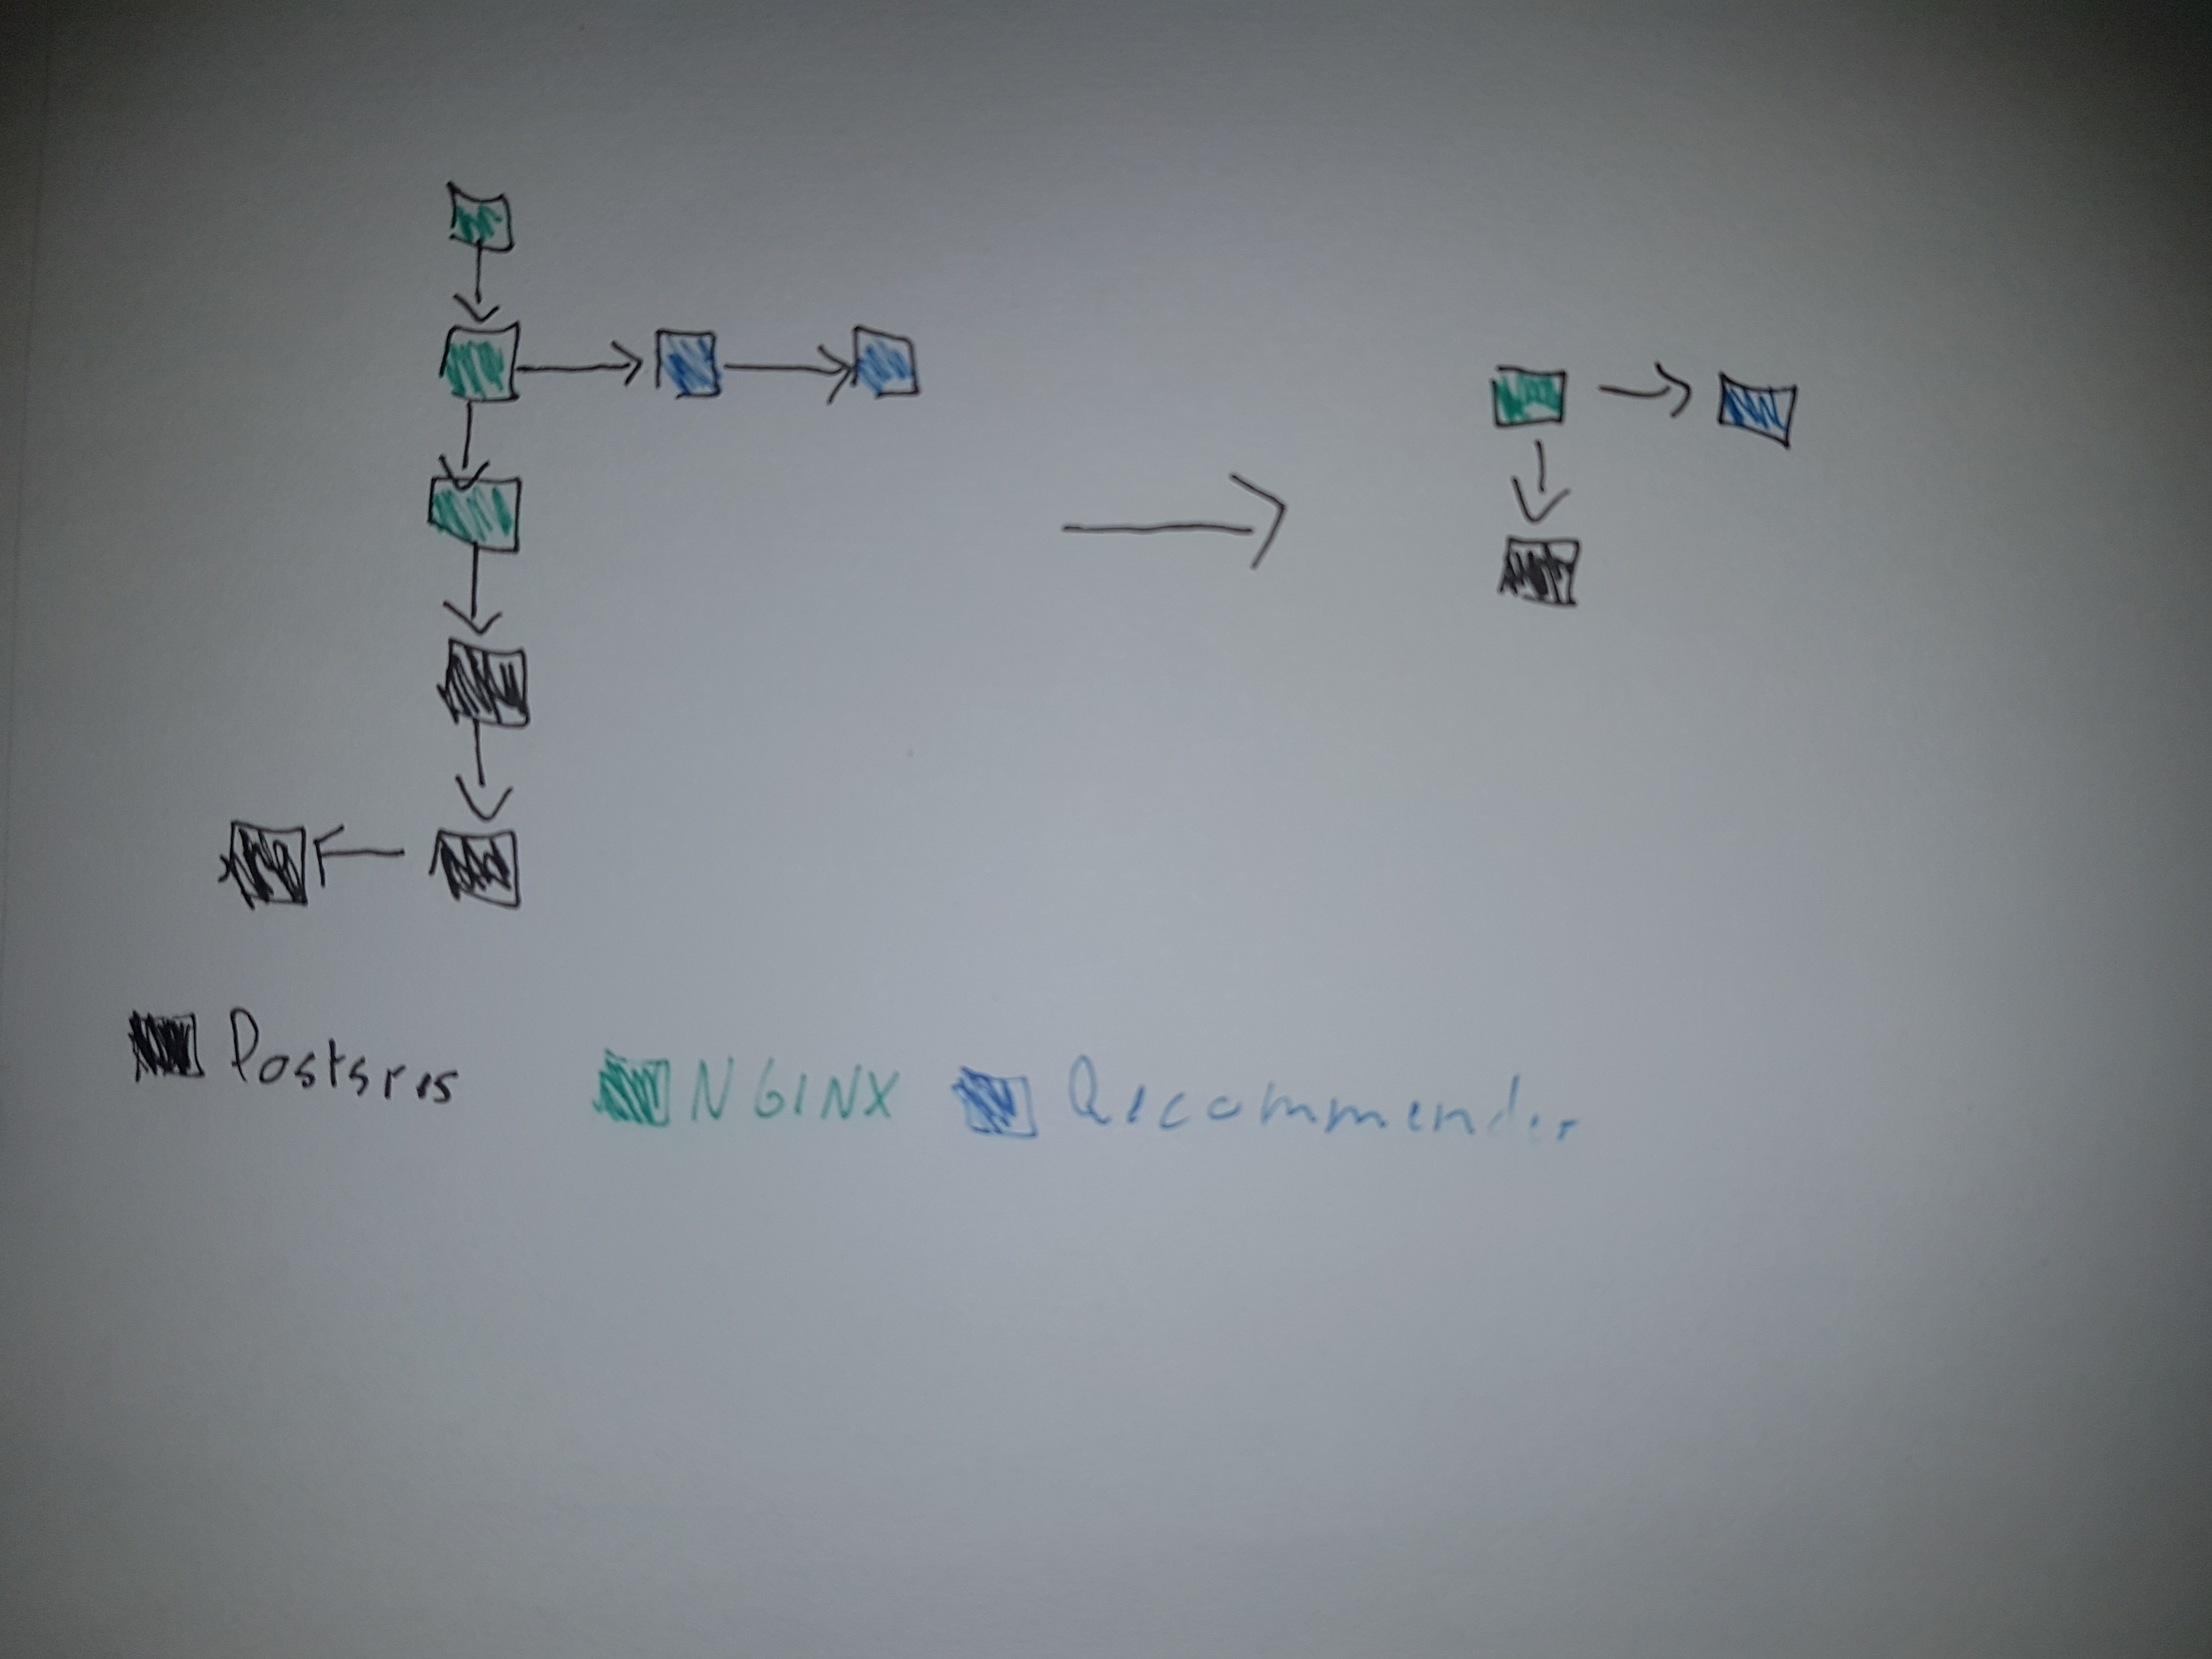
\includegraphics[width=\linewidth]{agg.jpg}
    \caption{Example of an aggregation task where events with the same \textit{process\_name} get aggregated into the same node.}
    \label{fig:aggregation}
\end{figure}
